\section{Interacción con el blanco}
\subsection{¿Que es una imagen SAR?}
\begin{frame}{} \vskip0cm
  \begin{columns}[t]
    \begin{column}{0.5\textwidth}
     \begin{block}{SAR}
       \begin{itemize}
         \item Una imagen SAR es un mapa de reflectividad.
         \item Indica cuanta energía vuelve al sensor.
         \item La cantidad de energía retrodispersada depende de la geometría del blanco y su conductividad eléctrica.
         \item Las zonas oscuras y brillantes son zonas de baja y alta reflectividad.
       \end{itemize}
     \end{block}
    \end{column}
    \begin{column}{0.5\textwidth}  %%<--- here
        \begin{figure}
          \centering
          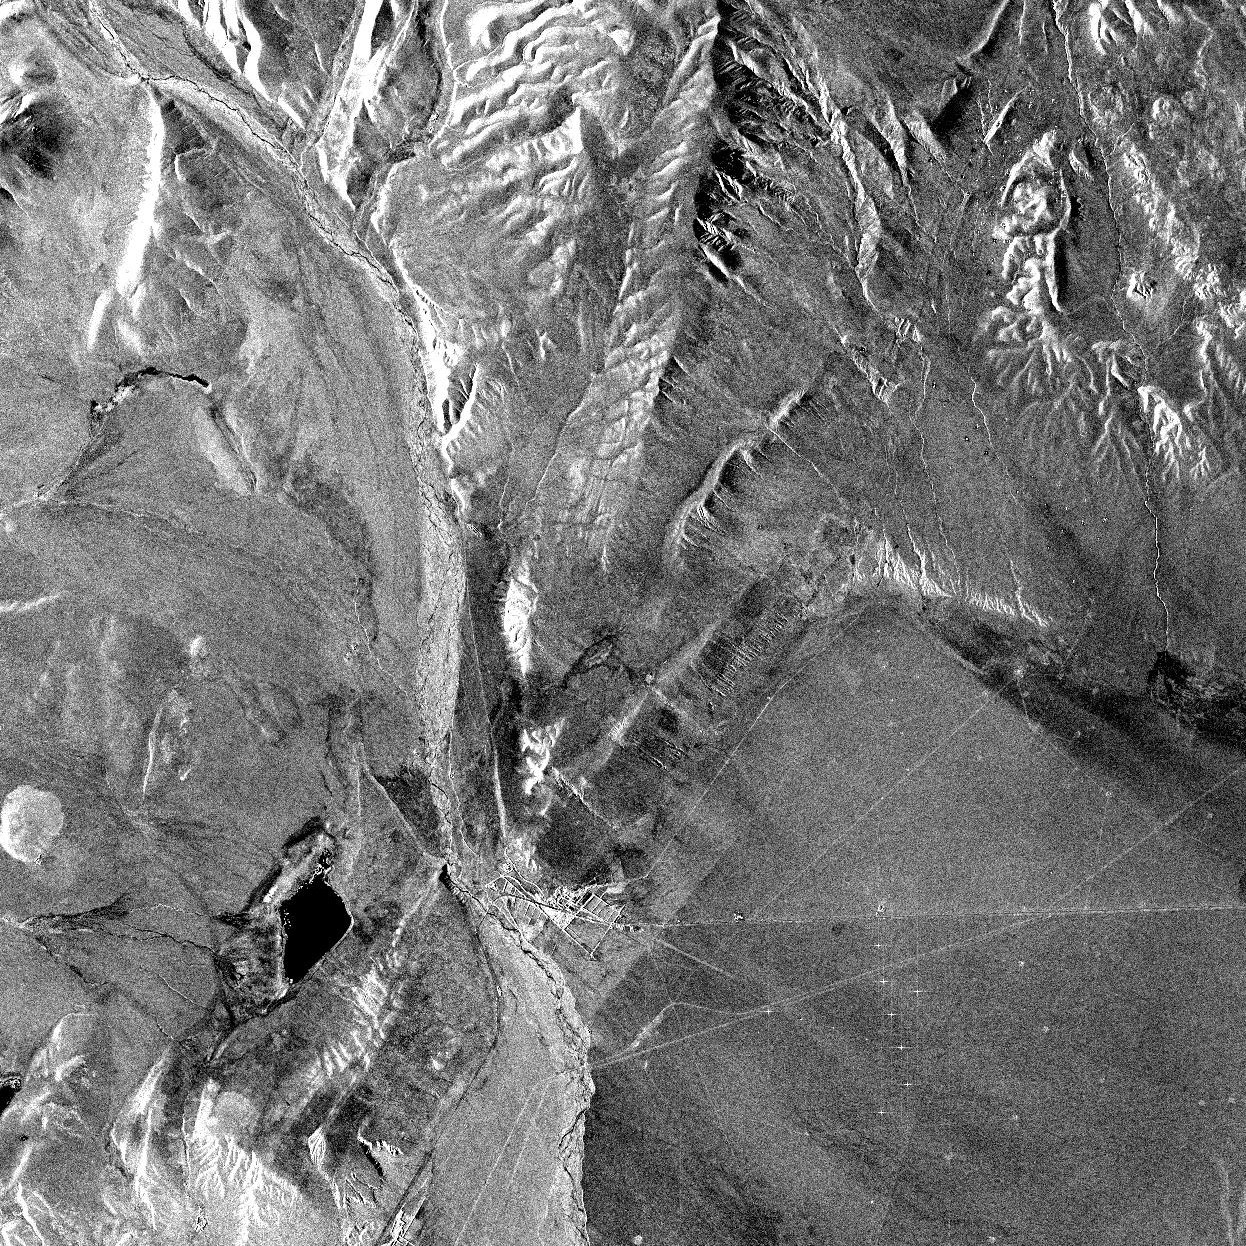
\includegraphics[width=0.8\textwidth]{fig:sar.jpg}
          \caption{Imagen SAR de una zona montañosa.}
          \label{}
        \end{figure}
    \end{column}
    \end{columns}
\end{frame}
%--- Next Frame ---%

\begin{frame}{} \vskip0cm
    \begin{figure}
      \centering
      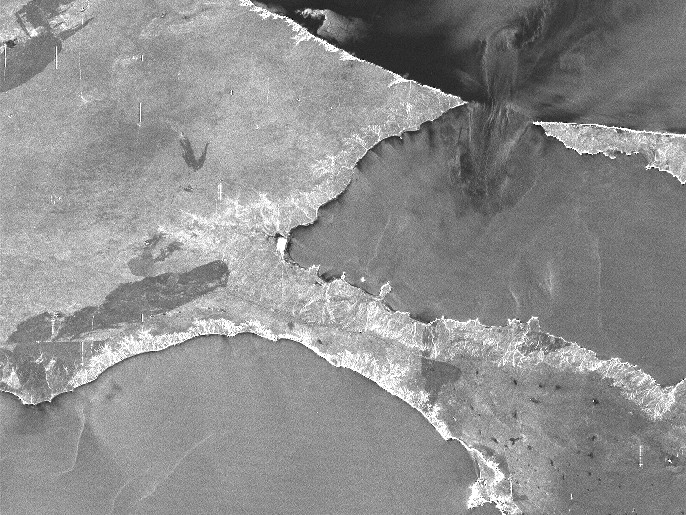
\includegraphics[width=0.6\textwidth]{fig:sar2.jpg}
      \caption{Imagen SAR de una región costera.}
      \label{}
    \end{figure}
\end{frame}
%--- Next Frame ---%

\subsection{Mecanismos de scattering}

\begin{frame}{} \vskip0cm
    \begin{figure}
      \centering
      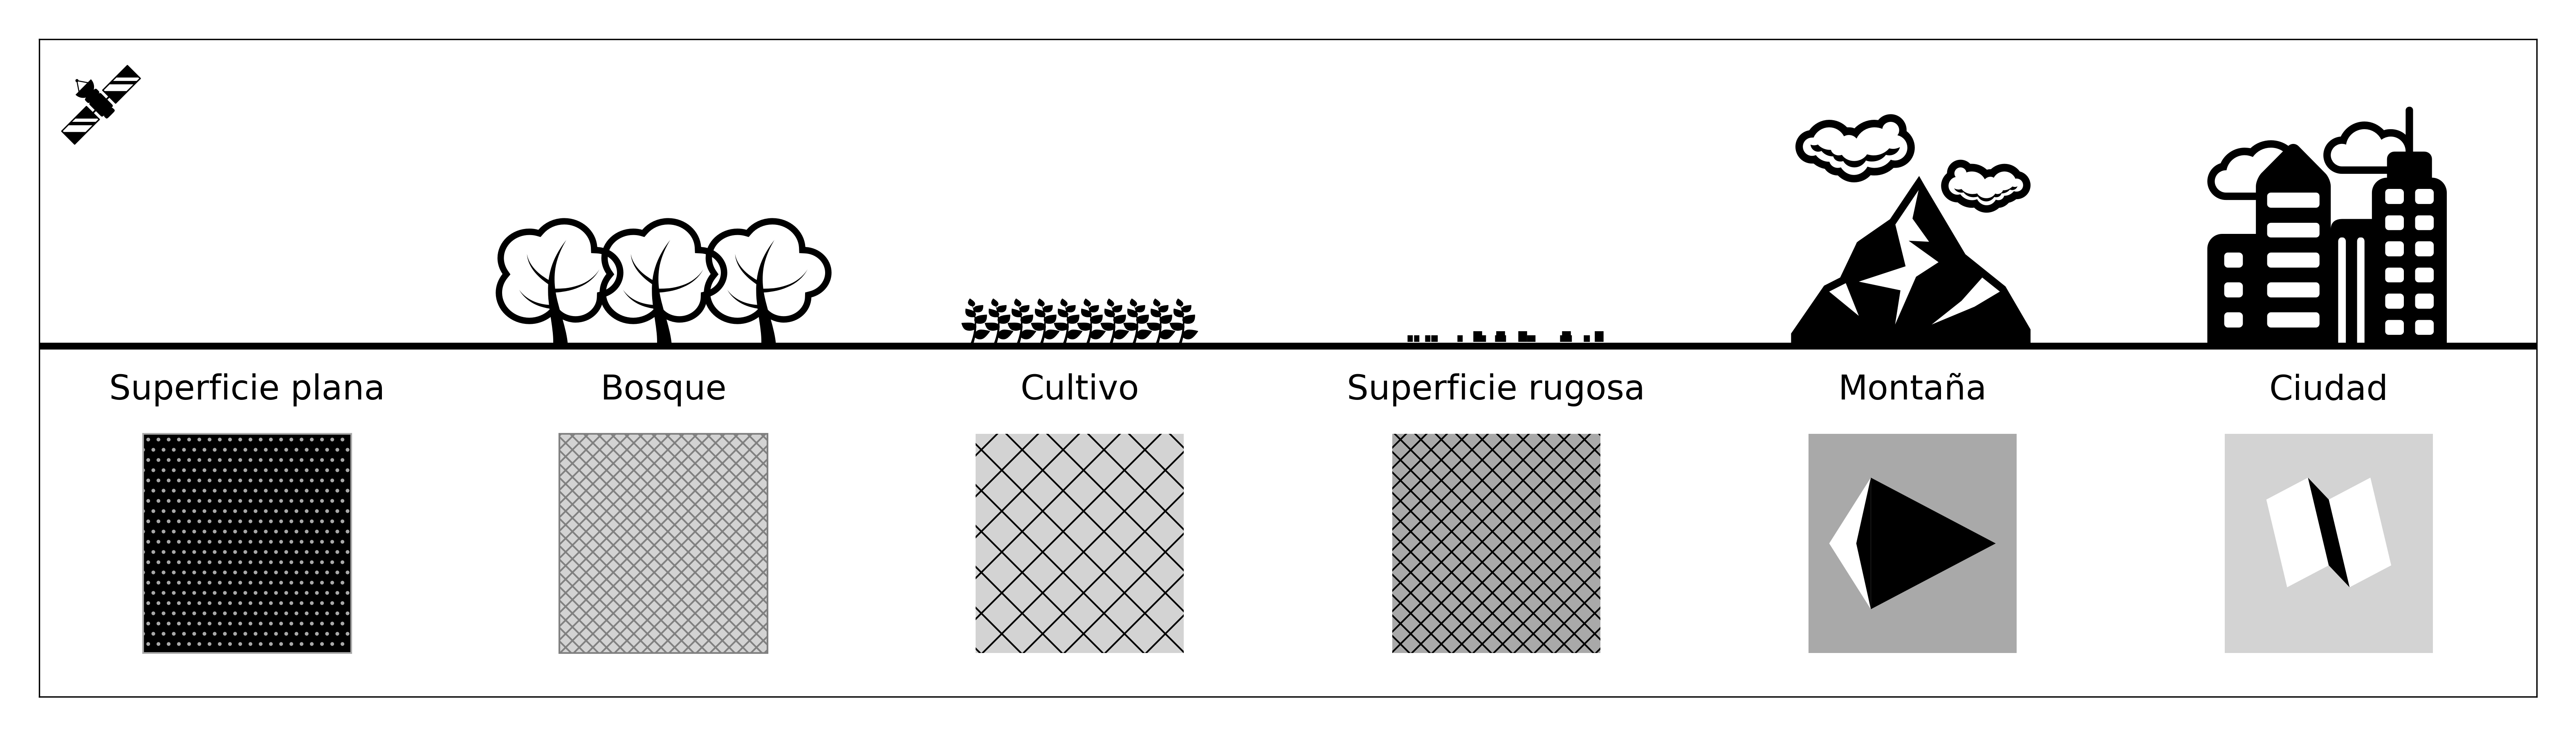
\includegraphics[width=\textwidth]{fig:blancos.png}
      \caption{Interpretación visual de distintos blancos en una imagen SAR considerando tono y textura. Pueden verse los mecanismos de interacción especular, en volumen y doble rebote.}
      \label{}
    \end{figure}
\end{frame}
%--- Next Frame ---%

\begin{frame}{} \vskip0cm
    \begin{figure}
      \centering
      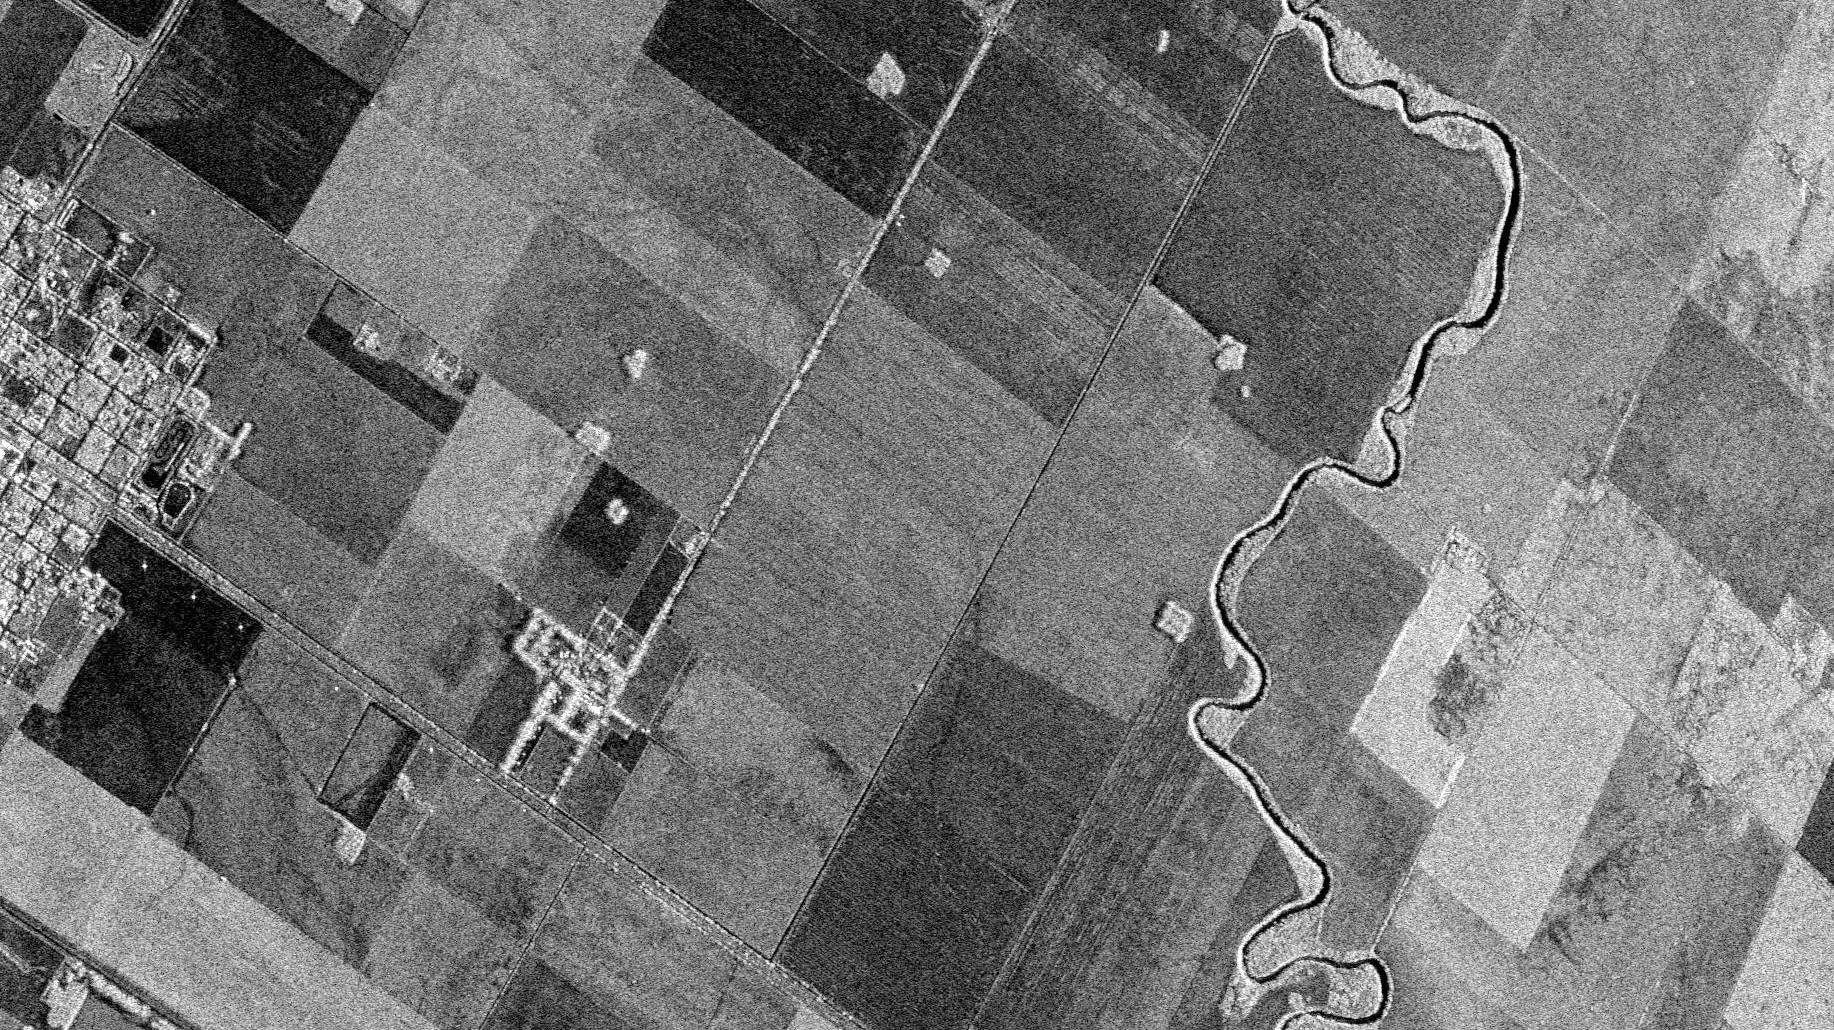
\includegraphics[width=0.6\textwidth]{fig:rebotes2.jpg}
      \caption{Imagen SAR de un área con cultivos. Pueden observarse varios de los mecanismos de interacción anteriores.}
      \label{}
    \end{figure}
\end{frame}
%--- Next Frame ---%

\begin{frame}{} \vskip0cm
  \begin{figure}
    \centering
    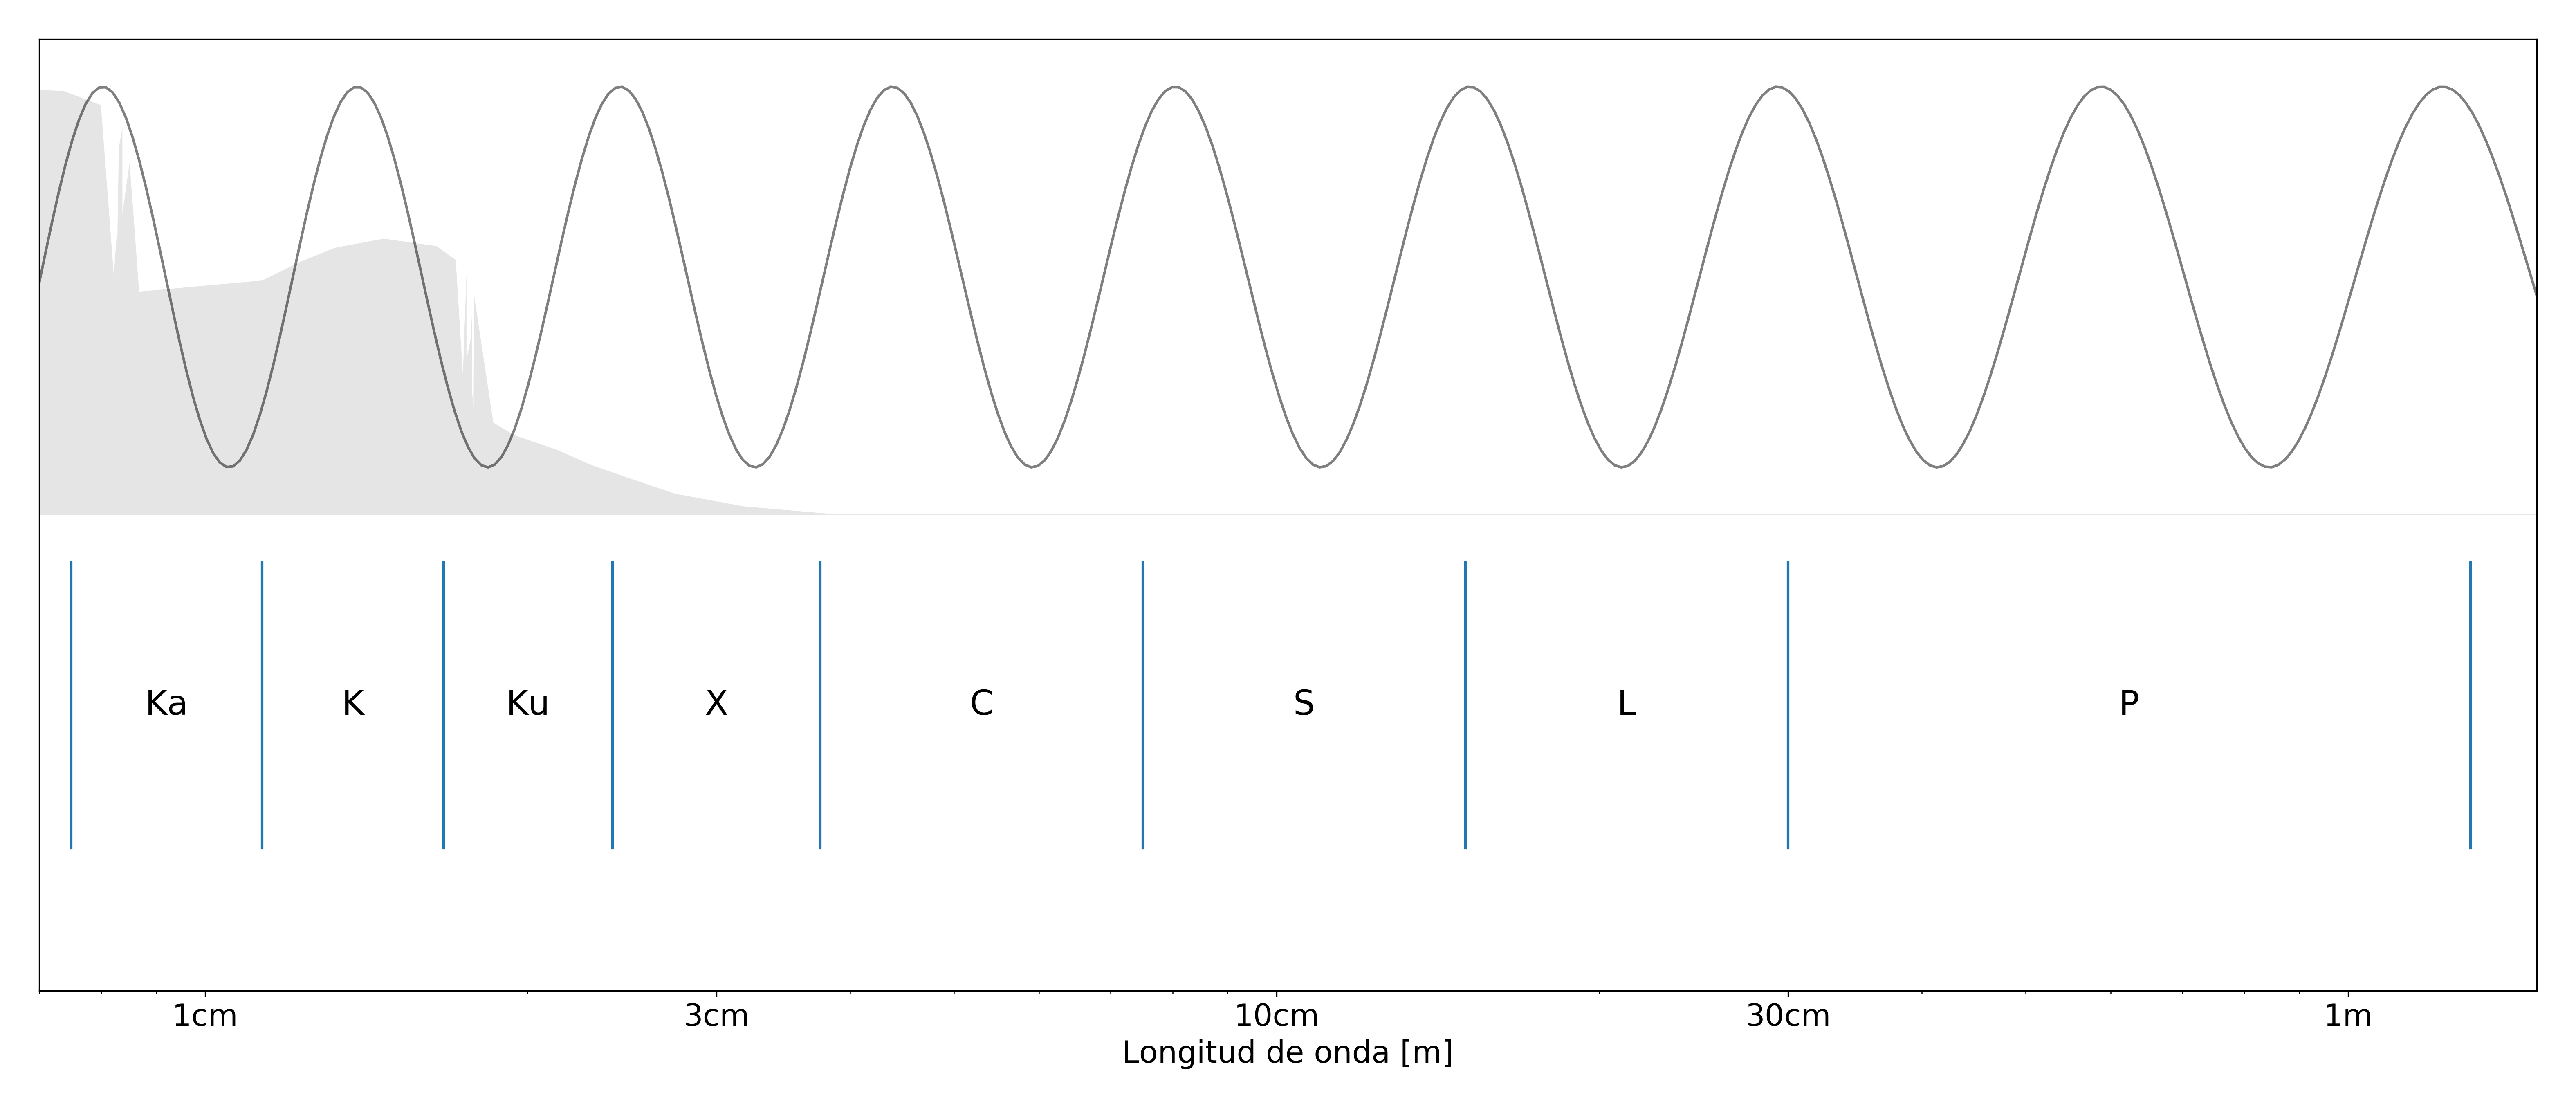
\includegraphics[width=\textwidth]{fig:espectrozoom.png}
    \caption{Espectro electromagnético en longitud de onda para la región de las microondas.}
    \label{}
  \end{figure}
\end{frame}
%--- Next Frame ---%

%\begin{frame}{} \vskip0cm
%    \begin{figure}
%      \centering
%      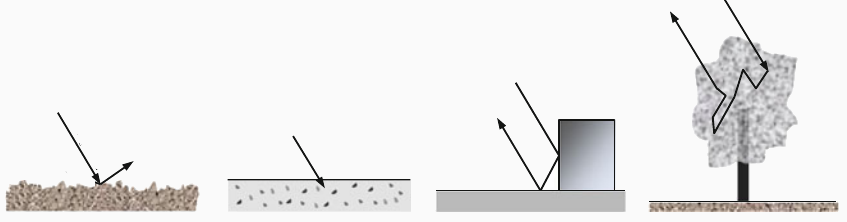
\includegraphics[width=0.9\textwidth]{fig:interacciones.png}
%      \caption{Interacciones entre los distintos blancos según la longitud de onda. De izquierda a derecha: especular, absorción, doble rebote y en volumen.}
%      \label{}
%    \end{figure}
%\end{frame}
%--- Next Frame ---%

\begin{frame}{} \vskip0cm
    \begin{figure}
      \centering
      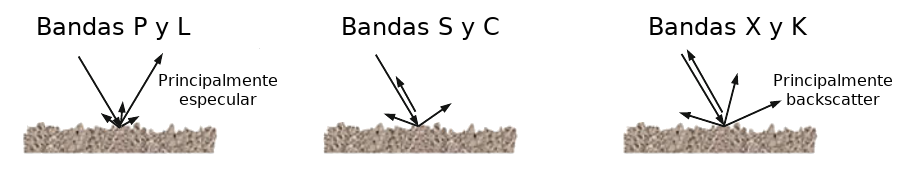
\includegraphics[width=\textwidth]{fig:interacciones-1.png}
      \caption{Interacciones entre los distintos blancos según la longitud de onda.}
      \label{}
    \end{figure}
\end{frame}
%--- Next Frame ---%

\begin{frame}{} \vskip0cm
    \begin{figure}
      \centering
      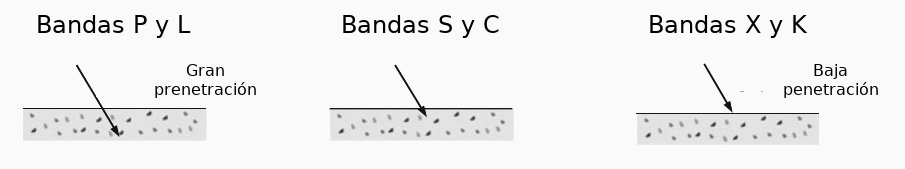
\includegraphics[width=\textwidth]{fig:interacciones-2.png}
      \caption{Interacciones entre los distintos blancos según la longitud de onda.}
      \label{}
    \end{figure}
\end{frame}
%--- Next Frame ---%

\begin{frame}{} \vskip0cm
    \begin{figure}
      \centering
      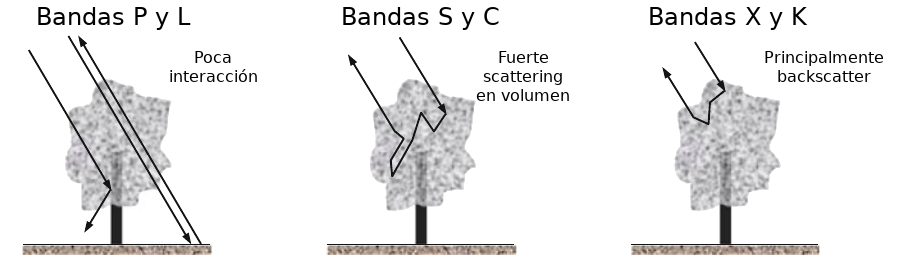
\includegraphics[width=\textwidth]{fig:interacciones-4.png}
      \caption{Interacciones entre los distintos blancos según la longitud de onda.}
      \label{}
    \end{figure}
\end{frame}
%--- Next Frame ---%

\begin{frame}{} \vskip0cm
    \begin{figure}
      \centering
      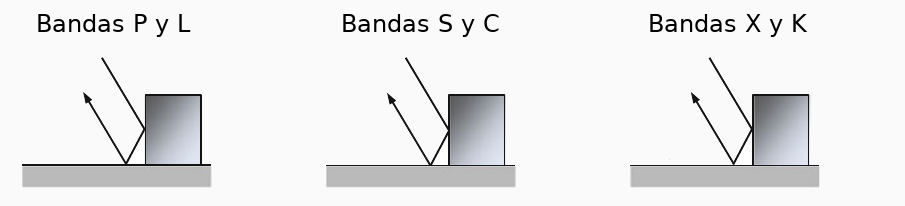
\includegraphics[width=\textwidth]{fig:interacciones-3.png}
      \caption{Interacciones entre los distintos blancos según la longitud de onda.}
      \label{}
    \end{figure}
\end{frame}
%--- Next Frame ---%




\begin{frame}{} \vskip0cm
    \begin{figure}
    \centering
    \subfloat[Banda C ($5.7cm$)]{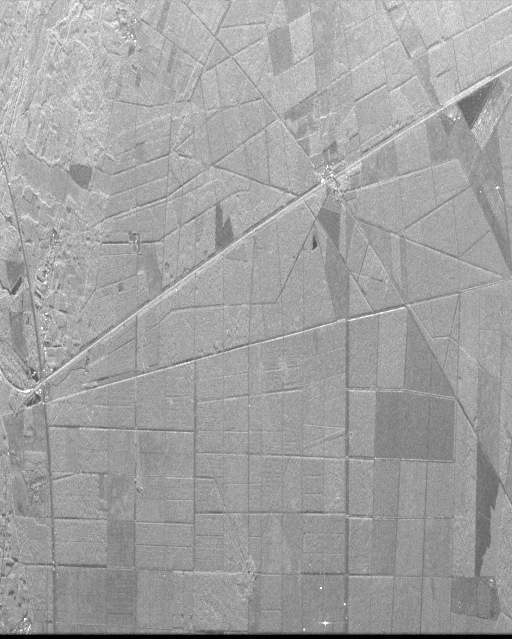
\includegraphics[width=0.2\textwidth]{fig:C.png}}\hspace{1cm}
    \subfloat[Banda L ($24cm$)]{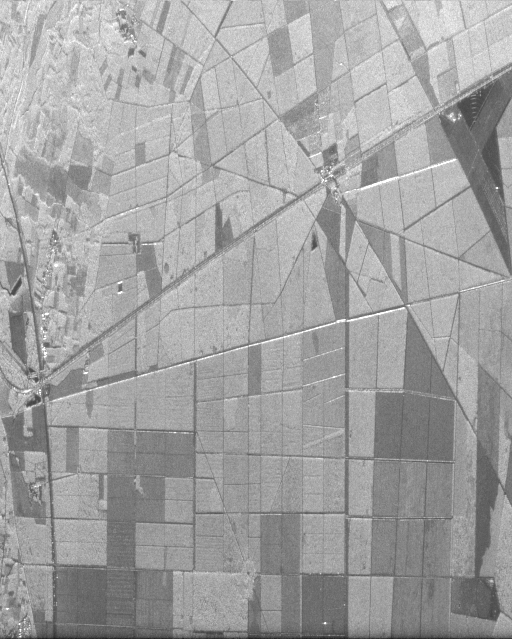
\includegraphics[width=0.2\textwidth]{fig:L.png}}\hspace{1cm}
    \subfloat[Banda P ($68cm$)]{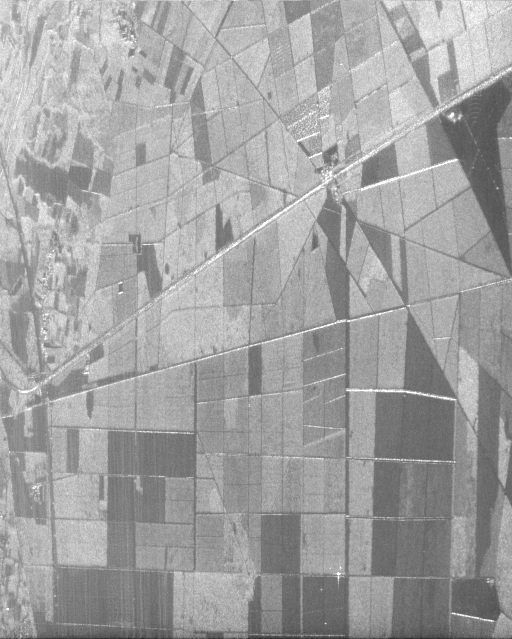
\includegraphics[width=0.2\textwidth]{fig:P.png}}
    \caption{Misma región vista en las bandas C, L y P.}
    \end{figure}
\end{frame}
%--- Next Frame ---%
\subsection{Resolución espacial}

\begin{frame}{} \vskip0cm
    A diferencia de la mayoría de los sistemas ópticos, los sistemas de radar tienen dos resoluciones:
    \begin{itemize}
      \item En rango, perdendicular a la dirección de movimiento del satélite.
      \item En acimut, paralelo a la dirección de movimiento del satélite.
    \end{itemize}
\end{frame}
%--- Next Frame ---%

\begin{frame}{} \vskip0cm
  Se calculan como:
    \begin{columns}
    \begin{column}{0.5\textwidth}
     \begin{block}{Resolución en rango}
      \begin{equation}
        \rho_{RG} = \frac{c}{2B}
      \end{equation}
     \end{block}
    \end{column}
    \begin{column}{0.5\textwidth}  %%<--- here
      \begin{block}{Resolución en azymuth}
        \begin{equation}
          \rho_{AZ} = \frac{L}{2}
        \end{equation}
      \end{block}
    \end{column}
    \end{columns}
    con $c$ la velocidad de la luz, $B$ el \emph{bandwidth} del sistema y $L$ la longitud de la antena.

    \begin{block}{Observación:}
      A diferencia de los satélites ópticos, la resolución en un sistema SAR no depende de la distancia entre el satélite y el blanco.
    \end{block}
\end{frame}
%--- Next Frame ---%


%\gracias
%--- Next Frame ---%
